\subsubsection{Zmniejszanie i partycjonowanie grafu za pomocą algorytmu LAM}

Aby stworzyć mniejszy odpowiednik wejściowego grafu aplikowany jest algorytm tworzący skojarzenia (ang. matching).
Skojarzenie to podzbiór krawędzi grafu (ozn. $M$) o tej własności, że każdy wierzchołek jest końcem co najwyżej jednej krawędzi z $M$.
Pary wierzchołków połączone bezpośrednio krawędzią należącą do $M$ są skojarzone przez $M$ \cite{wiki:skojarzenie}.
\begin{figure}[h]
    \centering
    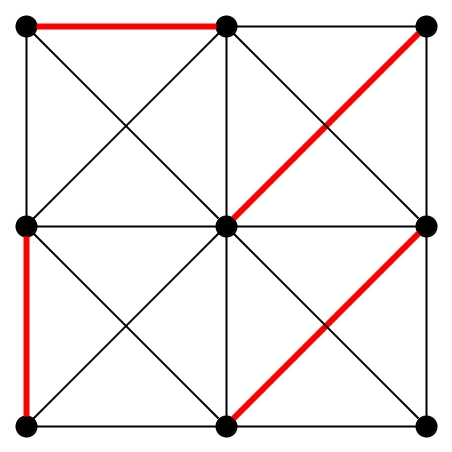
\includegraphics[width=0.24\linewidth]{images/Maximum_matching}
    \caption{Skojarzenie największe, którego liczba krawędzi wynosi 4.
    Źródło: \cite{wiki:skojarzenie}.}
    \label{im:max_skojarzenie}
\end{figure}

W celu zmniejszenia grafu aplikowana jest heurystyka, która bazuje na metodzie \cite{weighted_maching}.
Algorytm ten oblicza $2$-approximation dla problemu maximum weighted matching w czasie liniowym.
Algorytm ten startuje od arbitralnej krawędzi i sprawdza sąsiednie krawędzie.
Tak, jak długo jest w stanie znaleźć sąsiednią
krawędź z wyższą wagą, algorytm wywołuje się na niej i powtarza tę procedure aż znajdzie krawędź z lokalnie najwyższą
wagą.
Ta krawędź łączy dwa wierzchołki, które zostaną skojarzone.
W ten sposób skonstruowany algorytm dąży do budowania obszarów, które są możliwie ''zwarte'',
innymi słowy oznacza to, że granice między obszarami są możliwie krótkie oraz niepostrzępione.
Krawędzie z wysokimi wagami to krawędzie między wierzchołkami,
które reprezentują zbiory wierzchołków, które w początkowym grafie miały między sobą długą granicę.
Proces działania algorytmu pokazany jest na rysunku \ref{im:lam_steps}.

\begin{figure}[h]
    \centering
    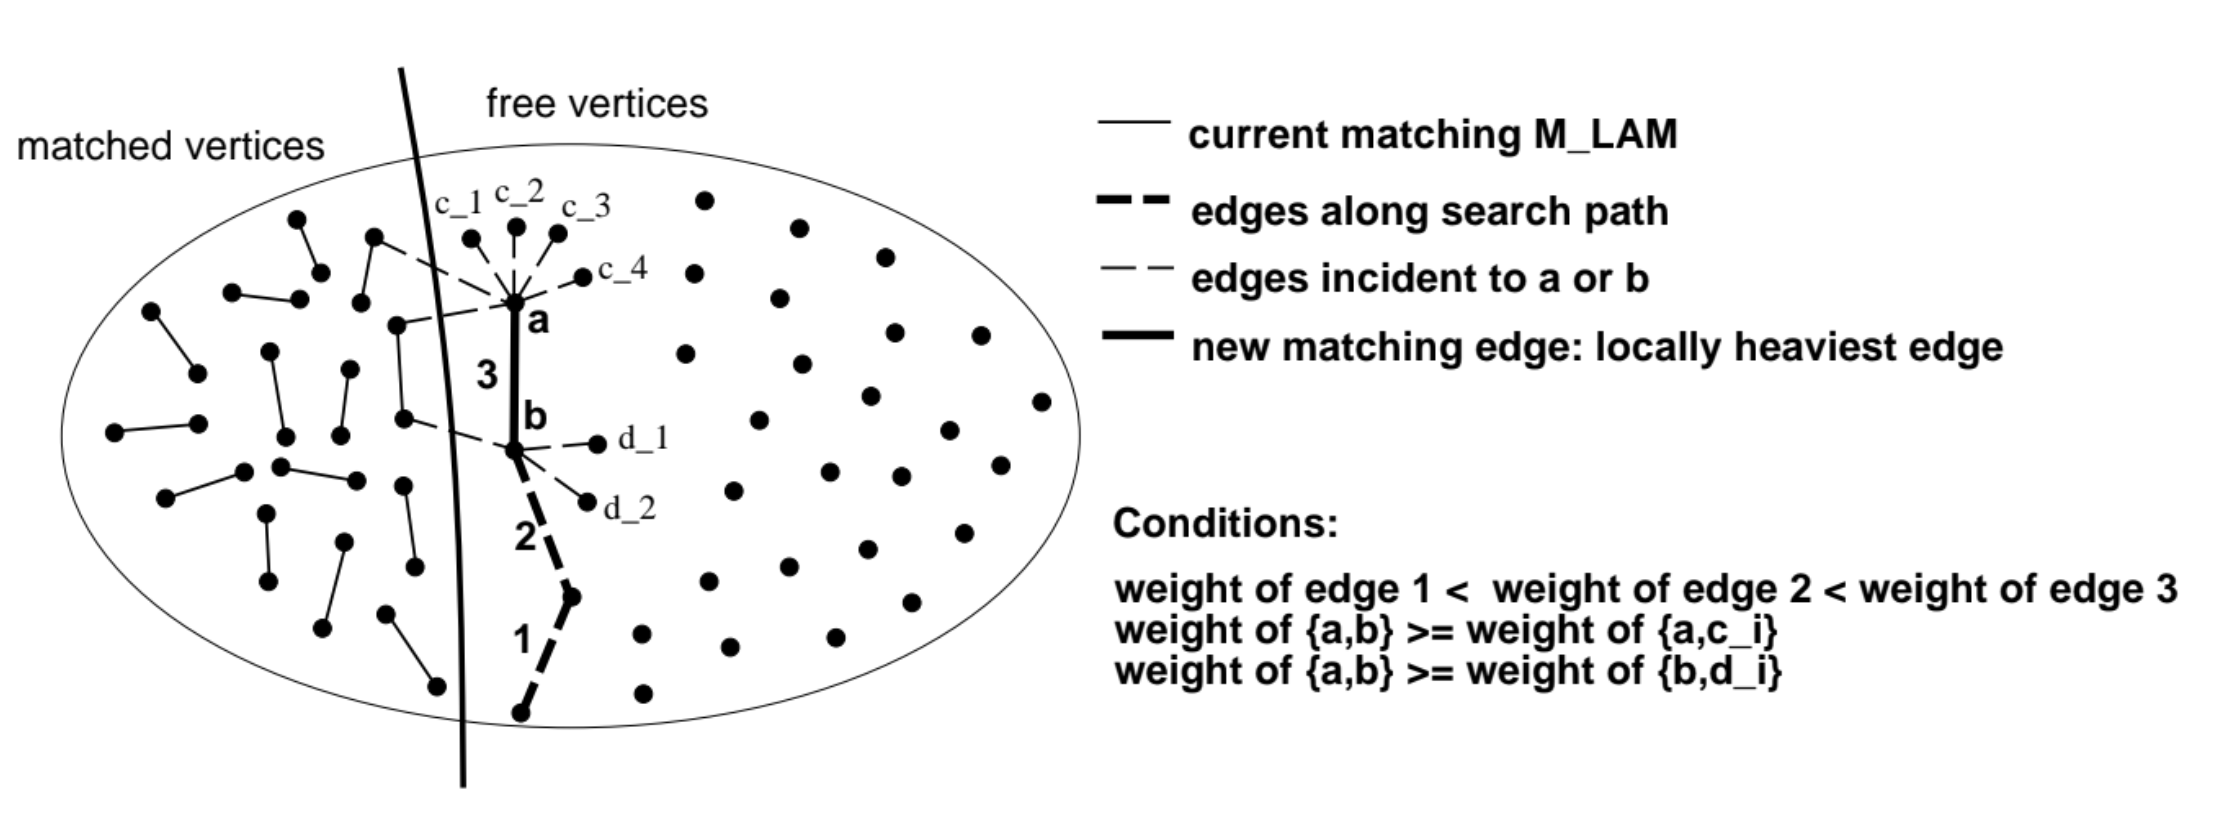
\includegraphics[width=0.9\linewidth]{images/lam}
    \caption{Fragment przebiegu algorytmu LAM. Startując z wybranej arbitralnie krawędzi numer 1, ścieżka buduje się
    przez krawędzie z lokalnie wyższymi wagami - krawędź numer 2 oraz 3 -
    aż do znalezienia krawędzi \(\{a, b\}\) z lokalnie największą wagą. (Pokazywane są tylko krawędzie z aktualnego
    wywołania algorytmu LAM, krawędzi znajdujące się na ścieżce oraz krawędzi sąsiadujące do \(\{a, b\}\).
    Źródło: \cite{weighted_maching}.}
    \label{im:lam}
\end{figure}

\newpage
\begin{pseudocode}
@\underline{PROCEDURE shrink graph $(G)$}@
  t = 0 /* number of episodes */
  WHILE $|V_{G}|$ $\neq$ number of partitions we want to achieve
    matched_vertices = run LAM-Algorithm on $G$
    shrink $G$ based on the matched_vertices
    t = t + 1
  ENDWHILE


@\underline{LAM-Algorithm}@
  $M_{LAM} := \emptyset$; /* empty matching at the start */
  $U := E$; /* all edges are unchecked at the start */
  WHILE $(U \neq \emptyset)$
    take arbitrary edge $\{a,b\} \in U$;
    try match $(\{a,b\})$;
  ENDWHILE


@\underline{PROCEDURE try match $(\{a,b\})$}@
  $C_{\{a,b\}}(a) := \emptyset;$ $ C_{\{a,b\}}(b) := \emptyset;$ /* empty local sets of checked edges at the start */
  WHILE $(a$ is free AND $b$ is free AND $(\exists \{a,c\} \in U$ OR $\exists \{b,d\} \in U))$
    IF $(a$ is free AND $\exists \{a,c\} \in U)$
      move $\{a,c\}$ from $U$ to $C_{\{a,b\}}(a)$; /* move from U to C */
      IF $(w(\{a,c\}) > w(\{a,b\}))$
        try match $(\{a,c\})$; /* call heavier edge */
      ENDIF
    ENDIF
    IF $(b$ is free AND $\exists \{b,d\} \in U)$
      move $\{b,d\}$ from $U$ to $C_{\{a,b\}}(b)$; /* move from U to C */
      IF $(w(\{b,d\}) > w(\{a,b\}))$
        try match $(\{b,d\})$; /* call heavier edge */
      ENDIF
    ENDIF
  ENDWHILE
  IF $(a$ is free AND $b$ is free AND $\{a,b\}$ can be matched$)$
    add $\{a,b\}$ to $M_{LAM}$  /* new matching edge $\{a,b\}$ */
  ELSE IF $(a$ is matched AND $b$ is free$)$
    move edges $\{ \{b,d\} \in C_{\{a,b\}}(b)$ $|$ d is free$\}$ back to $U$;
  ELSE IF $(b$ is matched AND $a$ is free$)$
    move edges $\{ \{a,c\} \in C_{\{a,b\}}(a)$ $|$ c is free$\}$ back to $U$;
  ENDIF
\end{pseudocode}
\vspace{-8mm}
\captionof{listing}{Kod przedstawiający ulepszony algorytm LAM.
Wprowadzone przeze mnie zmiany dotyczyły warunku skojarzenia wierzchołków oraz końcowych
instrukcji warunkowych, które mogły zostać uproszczone z racji na brak potrzeby tworzenia zbioru krawędzi do usunięcia - $R$.
Niezmodyfikowany kod algorytmu można znaleźć w artykule \cite{weighted_maching}.}
\label{code:lam}
\newpage
Algorytm \ref{code:lam} przedstawia procedury służące do zmniejszania grafu.
Jest to algorytm opisany w \cite{weighted_maching}.
Końcowe efekty jego działania można obserwować na rysunku \ref{im:lam2} oraz \ref{im:lam_indivisible}.
Został ulepszony o bardziej rozbudowany warunek na łączenie wierzchołków oraz uproszczony o zbiór $R$, odpowiedzialny
za przechowywanie krawędzi do usunięcia.
Startuje z pustym zbiorem skojarzeń $M_{LAM}$.
Zbiór $U$ przechowuje nieodwiedzone krawędzie ($U = E$ na starcie).
Główną częścią algorytmu jest pętla WHILE (linia numer 13), która wywołuje
procedurę 'try match' z arbitralnie wybraną, nieodwiedzoną krawędzią $\{a,b\}$.
Ta krawędź nie jest dodawana do
zbioru skojarzeń dopóki wszystkie sąsiednie krawędzie prowadzące do wolnych wierzchołków (ang. free vertices) nie są sprawdzone
w poszukiwaniu nowej krawędzi z wyższą wagą - następuje to w pętli WHILE w linii numer 21.
Każde wywołanie procedury 'try match $(\{a,b\})$' przechowuje swoje własne zbiory lokalnie odwiedzonych krawędzi
$C_{\{a,b\}}(a)$ oraz $C_{\{a,b\}}(b)$, w zależności od tego czy nieodwiedzone krawędzie są sąsiadujące z wierzchołkiem
$a$ czy z $b$.
Jeśli wierzchołki $a$ i $b$ są wolne oraz co najmniej jeden z nich jest wierzchołkiem należącym do jednej z
nieodwiedzonych krawędzi, nieodwiedzona krawędź jest sprawdzana dalszymi instrukcjami.
Jeśli ma wyższą wagę od krawędzi $\{a,b\}$, 'try match' wywołuje się na niej rekursywnie.
Rekursywne wywołania są powtarzane aż do znalezienia krawędzi z lokalnie najwyższą wagą.
Następnie krawędź dodawana jest do $M_{LAM}$, a algorytm zakończa aktualne wywołanie 'try match' i kontynuuje
pętlę WHILE sprawdzając kolejne sąsiadujące krawędzie.
Pętla WHILE zakończa się wtedy, gdy $a$ oraz/lub $b$ zostaną skojarzone w rekursywnym wywołaniu lub jeśli nie mają więcej
sąsiednich, nieodwiedzonych krawędzi. Następnie w końcowej części składającej się z instrukcji warunkowych
następuje sprawdzenie czy $a$ oraz $b$
są wolne. Jeśli tak, to $\{a,b\}$ jest dodawane do $M_{LAM}$.
W tej części, w oryginalnym algorytmie uzupełniany jest zbiór
wierzchołków do usunięcia \cite{weighted_maching} - $R$.
Ponadto jeśli $a$ lub $b$ są wolne to wszystkie krawędzie, które zostały
odwiedzone w aktualnym wywołaniu, zawierające w sobie wierzchołek $a$ lub $b$, zostają oznaczone jako nieodwiedzone -
są przenoszone do zbioru $U$.

\begin{figure}[h]
\centering
\begin{subfigure}{.5\textwidth}
    \centering
    \fbox{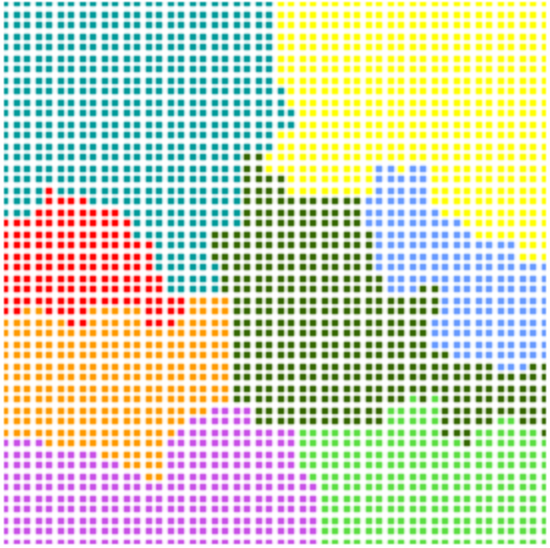
\includegraphics[width=0.6\linewidth]{images/lam-partitioning}}
    \caption[short]{partycjonowanie 1}
\end{subfigure}%
\begin{subfigure}{.5\textwidth}
    \centering
    \fbox{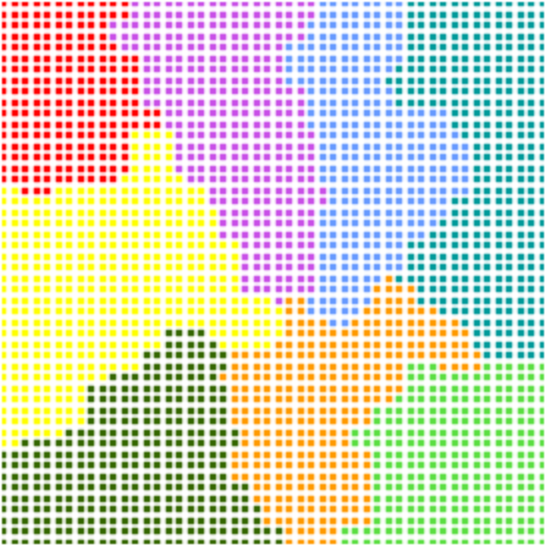
\includegraphics[width=0.6\linewidth]{images/lam-partitioning2}}
    \caption[short]{partycjonowanie 2}
\end{subfigure}
\caption{Dwa losowo wybrane partycjonowania siatki 50x50 na 8 obszarów za pomocą samego algorytmu LAM - bez fazy ulepszania podziału.
    Granice podziałów nie są optymalne, pola obszarów nie są równe - podział jest jednak bliski bycia równym w kwestii pól co jest
    oczekiwaną i dobrą bazą do dalszych operacji. Algorytm ma charakterystykę losową, to znaczy, że każde wywołanie
    będzie dawać inny rezultat. Zawsze jednak zachowane będzie dążenie do równych i zwartych obszarów.}
\label{im:lam2}
\end{figure}

Pętla WHILE w 21 linii sprawdza krawędzie sąsiadujące z wierzchołkiem $a$ oraz $b$ tylko jeśli obydwa wierzchołki są wolne.
Ta cecha jest używana przez autorów artykułu do udowodnienia liniowej złożoności algorytmu.

Nieodwiedzone krawędzie zawarte w $U$ mają taką właściwość, że obydwa należące do nich wierzchołki są wolne.
Nowe krawędzie są przenoszone ponownie do $U$ w końcowej części z instrukcjami warunkowymi, ale tylko jeśli obydwa ich
wierzchołki są wolne.
Tak skonstruowany algorytm jest uruchamiany wielokrotnie przez procedurę 'shrink graph', aż do kiedy liczba
wierzchołków w grafie nie osiągnie liczby partycji, na które chcemy podzielić wejściową siatkę.
Po każdym wywołaniu algorytmu LAM uruchamiana jest procedura, która zamienia skojarzone pary wierzchołków na pojedyncze
wierzchołki wraz ze zmianą wagi.
Wyjątkiem jest ostatnie wywołanie, kiedy liczba wierzchołków w grafie osiąga wartość docelową.
Wtedy łączonych jest
pierwsze $n$ par wierzchołków, tak by otrzymać wymaganą liczbę wierzchołków.
Waga wierzchołka powstałego ze skojarzenia jest sumą wag wierzchołków kojarzonych.
Jeśli na skutek skojarzena powstaje krawędź,
która zastępuje kilka krawędzi to jej waga jest sumą wag tych krawędzi.
Następnie do wierzchołków przyporządkowywane są numery partycji.
Zwykle jedno wywołanie algorytmu LAM
tworzy liczbę skojarzeń niewiele mniejszą niż połowa liczby wierzchołków w grafie.
W ten sposób graf, szczególnie w początkowych wywołaniach, zmniejszany jest o około połowę po każdym wywołaniu algorytmu LAM.
\vspace{mm}
\begin{figure}[h]
\centering
\begin{subfigure}{.5\textwidth}
    \centering
    \fbox{
\includegraphics[width=0.8\textwidth]{images/lam-obszary-niepodzielne/grid}}
    \caption[short]{siatka do partycjonowania}
\end{subfigure}%
\begin{subfigure}{.5\textwidth}
    \centering
    \fbox{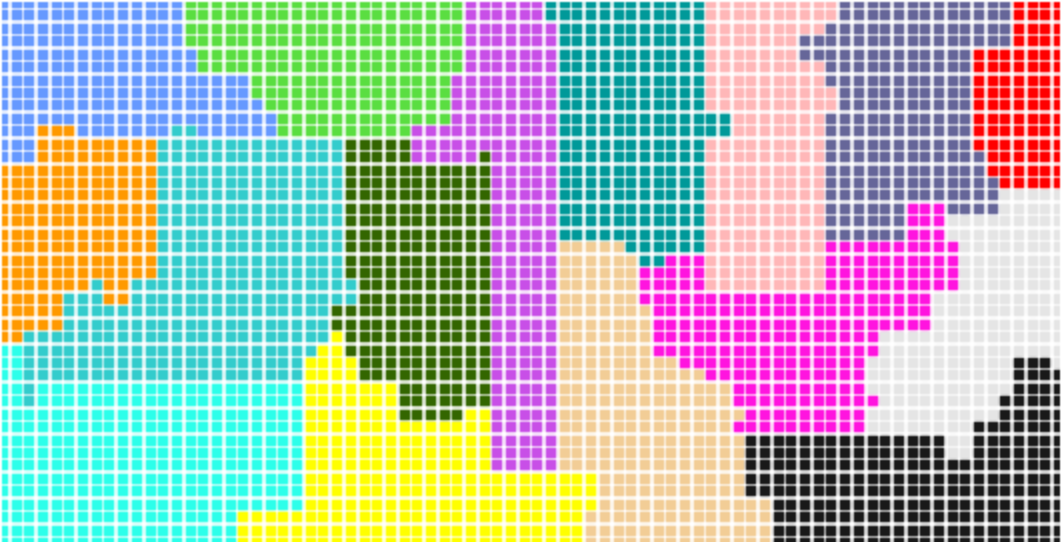
\includegraphics[width=0.8\textwidth]{images/lam-obszary-niepodzielne/4}}
    \caption[short]{partycjonowanie}
\end{subfigure}
\caption{Obrazek (b) przedstawia partycjonowanie siatki (a) samym algorytmem LAM. Widoczne jest uwzględnianie obszarów
niepodzielnych, które na siatce (a) zaznaczone są jako obszary żółte.}
\label{im:lam_indivisible}
\end{figure}

\newpage
\newcommand\imgs{0.43}
\begin{figure}[h]
\begin{subfigure}{.5\textwidth}
    \centering
    \fbox{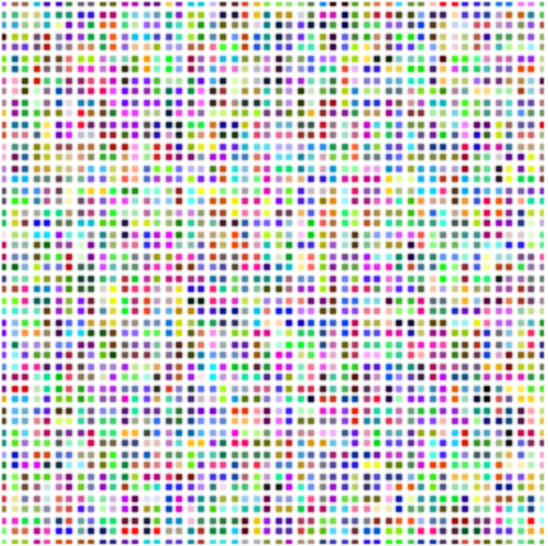
\includegraphics[width=\imgs\textwidth]{images/part-steps/lam1}}
    \caption[short]{krok 1}
\end{subfigure}
\begin{subfigure}{.5\textwidth}
    \centering
    \fbox{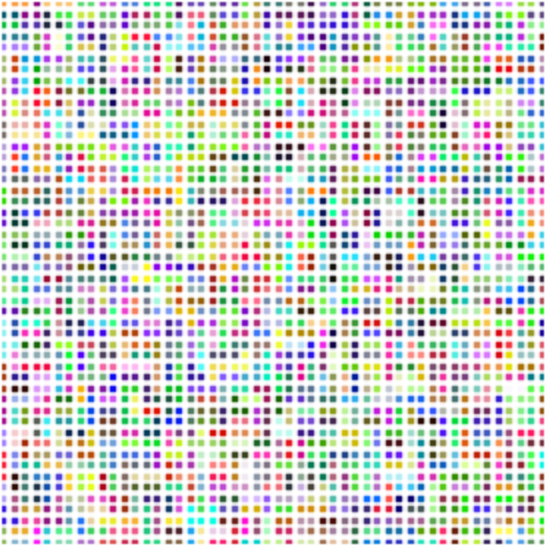
\includegraphics[width=\imgs\textwidth]{images/part-steps/lam2}}
    \caption[short]{krok 2}
\end{subfigure}%

\begin{subfigure}{.5\textwidth}
    \centering
    \fbox{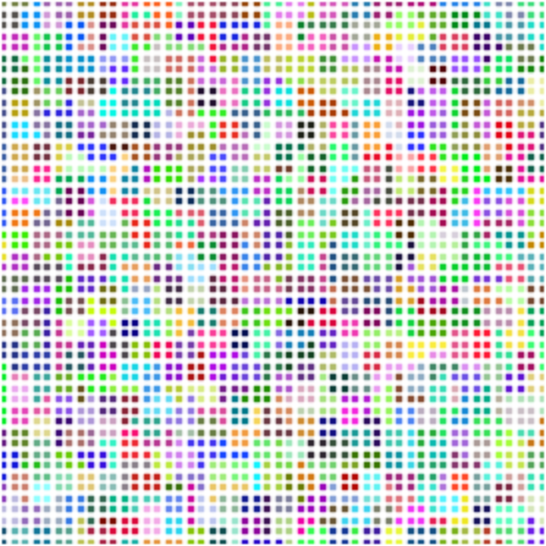
\includegraphics[width=\imgs\textwidth]{images/part-steps/lam3}}
    \caption[short]{krok 3}
\end{subfigure}
\begin{subfigure}{.5\textwidth}
    \centering
    \fbox{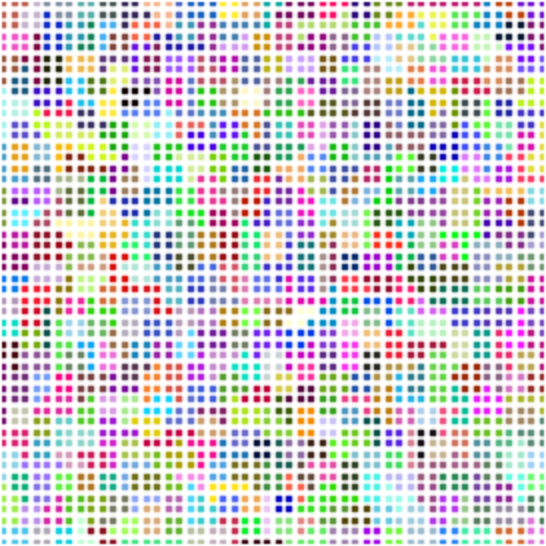
\includegraphics[width=\imgs\textwidth]{images/part-steps/lam4}}
    \caption[short]{krok 4}
\end{subfigure}%

\begin{subfigure}{.5\textwidth}
    \centering
    \fbox{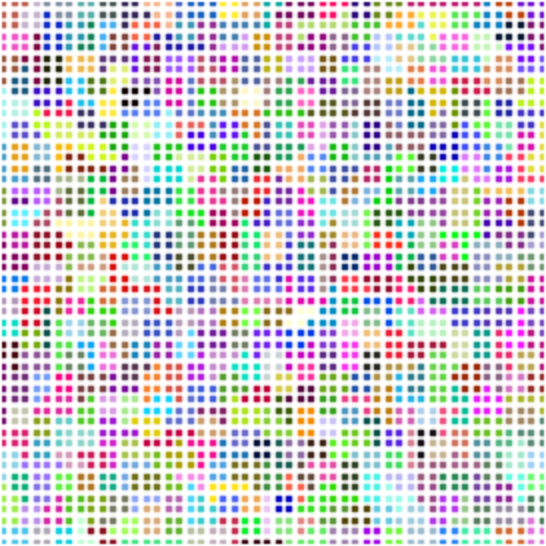
\includegraphics[width=\imgs\textwidth]{images/part-steps/lam5}}
    \caption[short]{krok 5}
\end{subfigure}
\begin{subfigure}{.5\textwidth}
    \centering
    \fbox{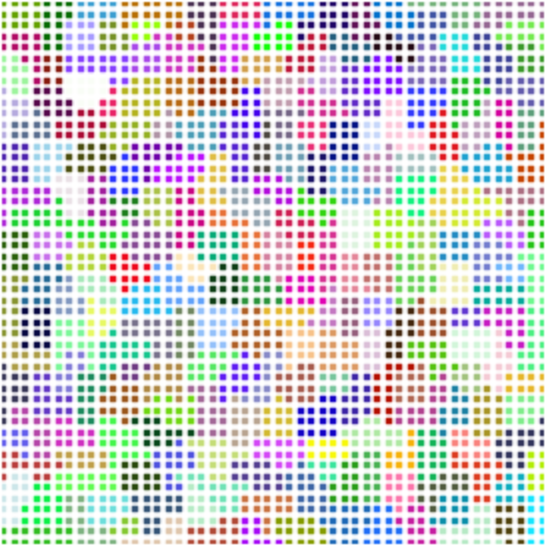
\includegraphics[width=\imgs\textwidth]{images/part-steps/lam6}}
    \caption[short]{krok 6}
\end{subfigure}%

\begin{subfigure}{.5\textwidth}
    \centering
    \fbox{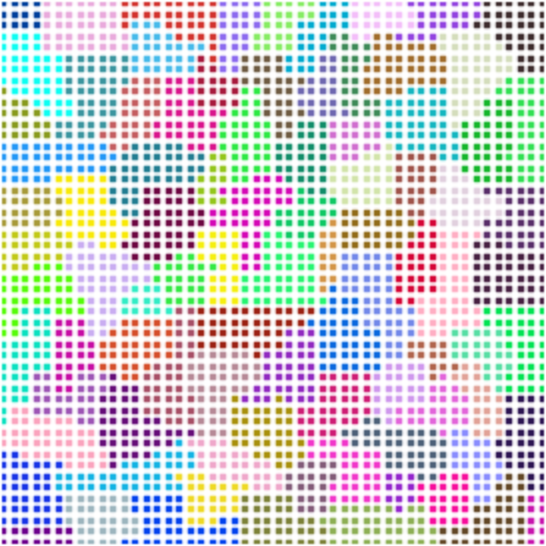
\includegraphics[width=\imgs\textwidth]{images/part-steps/lam7}}
    \caption[short]{krok 7}
\end{subfigure}
\begin{subfigure}{.5\textwidth}
    \centering
    \fbox{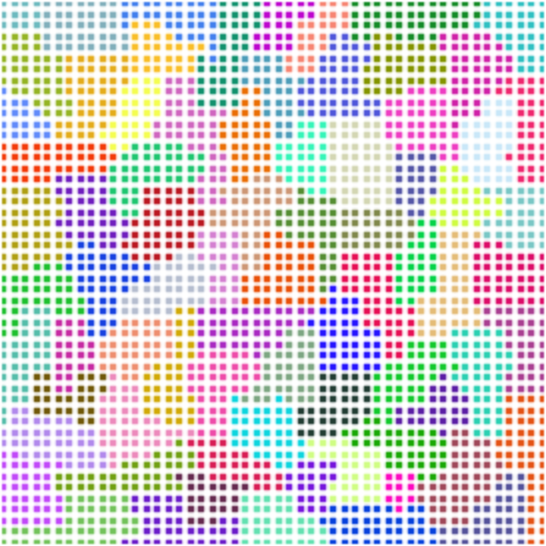
\includegraphics[width=\imgs\textwidth]{images/part-steps/lam8}}
    \caption[short]{krok 8}
\end{subfigure}%

\begin{subfigure}{.5\textwidth}
    \centering
    \fbox{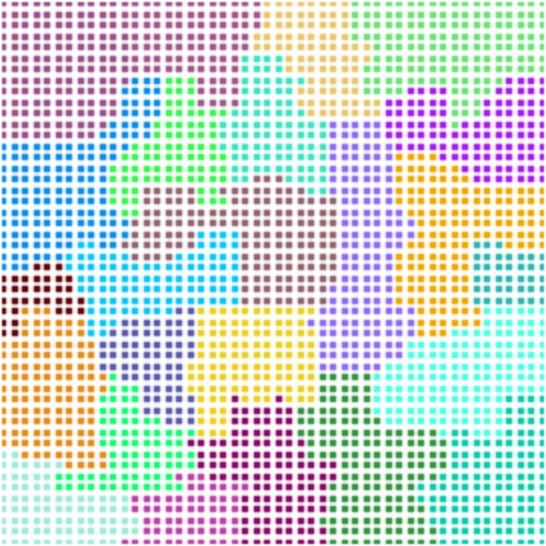
\includegraphics[width=\imgs\textwidth]{images/part-steps/lam9}}
    \caption[short]{krok 9}
\end{subfigure}
\begin{subfigure}{.5\textwidth}
    \centering
    \fbox{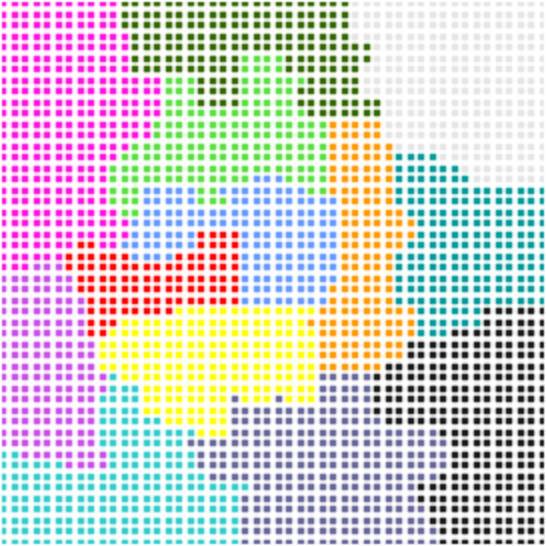
\includegraphics[width=\imgs\textwidth]{images/part-steps/lam10}}
    \caption[short]{krok 10}
\end{subfigure}
\caption{Obrazki przedstawiają wybrane, kolejne kroki algorytmu LAM aż do otrzymaniu podziału siatki 50x50 na 13 obszarów.
Nie są to wszystkie kroki. Rysowane było co
siódme wywołanie algorytmu oraz efekt końcowy. Widoczne jest równomierne łączenie obszarów.}
\label{im:lam_steps}
\end{figure}
\FloatBarrier